\section{Experimental Results}

\subsection{Methodology}
For our experiment, we test and compare the performance of all our algorithms over 3 difficulty-level based categories of datasets \cite{bib_rateddataset}. The difficulty levels are Easy, Medium, and Hard. Each of these categories are based on labelling by a human and each category has 10 puzzles.

We use the following methodology and evaluation criteria for the algorithms:
\begin{enumerate}
    \item We create the agents based on 4 algorithms: Backtracking, Convolutional Neural Networks, Constraint Satisfaction, and Genetic Algorithm.
    \item We run all the above mentioned agents on our difficulty-level based categorised datasets.
    \item We record the time taken to solve the puzzles in each category of datasets.
    \item We record the memory consumption for solving the puzzles in each category of datasets.
    \item We run and record the time taken and memory consumption for our baseline algorithm (Depth First Search) as well.
    \item We create tables for time and memory usage to compare the performance of all the algorithms against the baseline.
\end{enumerate}

\subsubsection{Note:} The memory consumption calculation is done based on \cite{bib_memoryeval}. It breaks down the memory usage into two categories:
\begin{enumerate}
    \item \textbf{RSS}: Resident Set Size, which is the physical memory used by a process (i.e. Stack + Heap memory).
    \item \textbf{VMS}: Virtual Memory Size, which is the virtual memory used by a process.
\end{enumerate}

\subsection{Results}

The following tables illustrate the results of our time and memory analysis by pitting the 4 of our chosen algorithms against the baseline of DFS algorithm:

\begin{figure} [htbp]
\centering
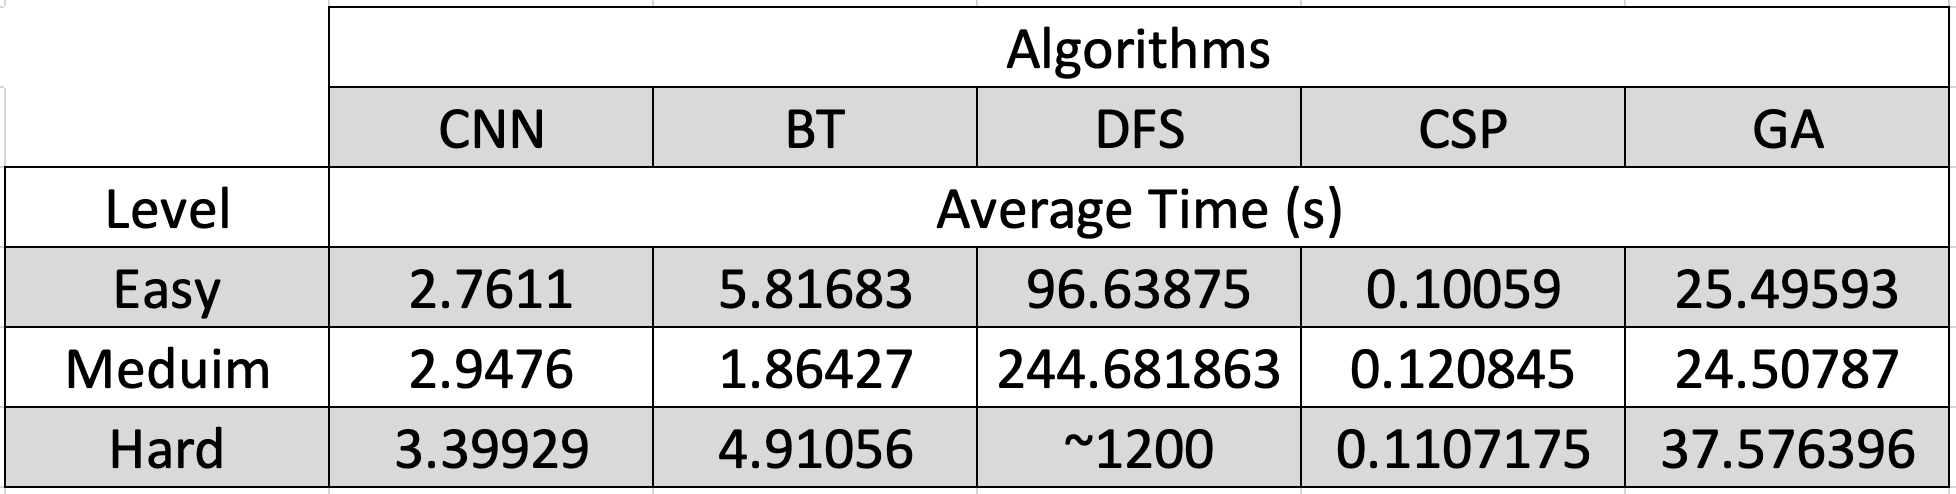
\includegraphics[width=90mm,scale=1]{figures/time-taken.png}
\caption{Average Time Taken to Solve Sudoku Puzzles of Various Difficulty Levels}
\label{fig:time_eval}
\end{figure}

\begin{figure} [htbp]
\centering
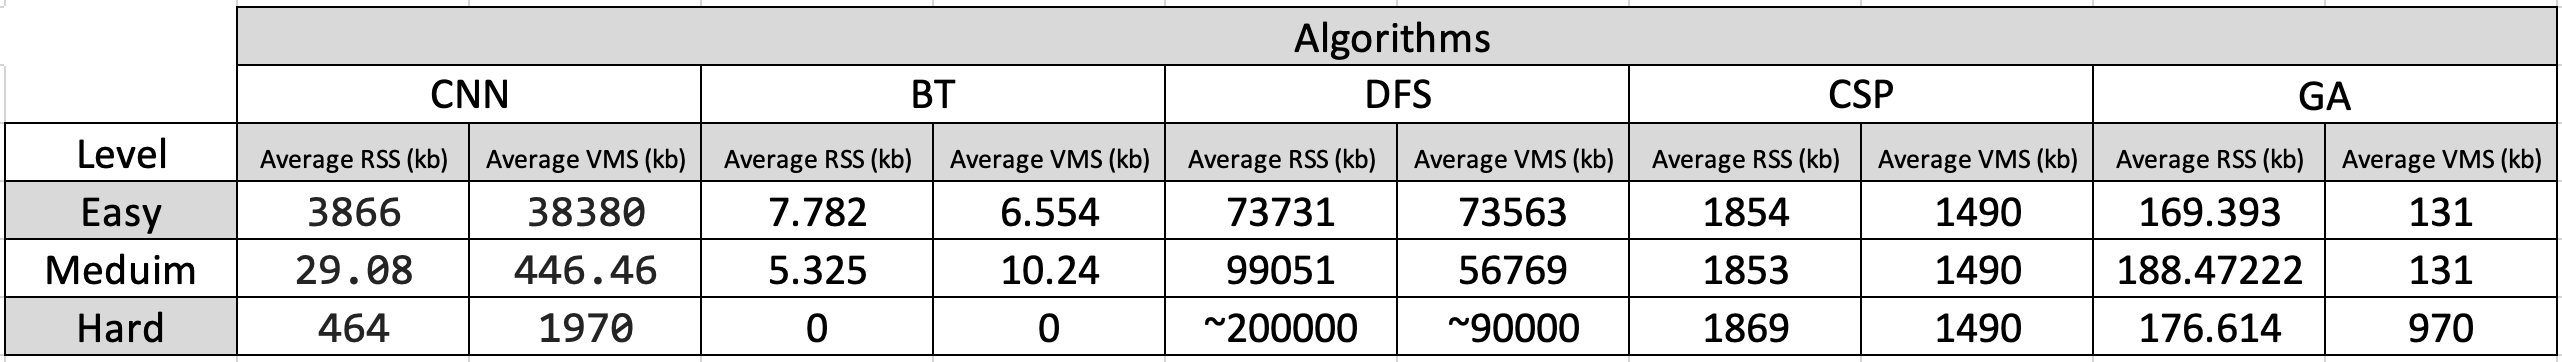
\includegraphics[width=120mm,height=30mm]{figures/memory-used.png}
\caption{Memory Used to Solve Sudoku Puzzles of Various Difficulty Levels; \centering RSS = Stack+Heap, VMS = Virtual Memory}
\label{fig:memory_eval}
\end{figure}

\subsection{Discussion}

\subsubsection{Backtracking:}
In our experiment, we discovered that certain problems are more difficult to be solved than others, even though the difficulty level is the same. We observed an anomaly as well. As can be seen in Fig. \ref{fig:backtrack_time}, it took 40 seconds to solve an easy Sudoku puzzle (more than any other puzzles with hard difficulty level) while most of the other easy puzzles took about one second to solve. A possible explanation for the anomaly is that since the backtracking algorithm strictly follows its process, what might be easy for a human being might not be easy for the algorithm. The easy, medium, and hard puzzles we have used were labelled with those difficulty levels by a human being. The backtracking algorithm, limited by its quirks, took the long route to solving the first "Easy" problem.

\begin{figure} [htbp]
\centering
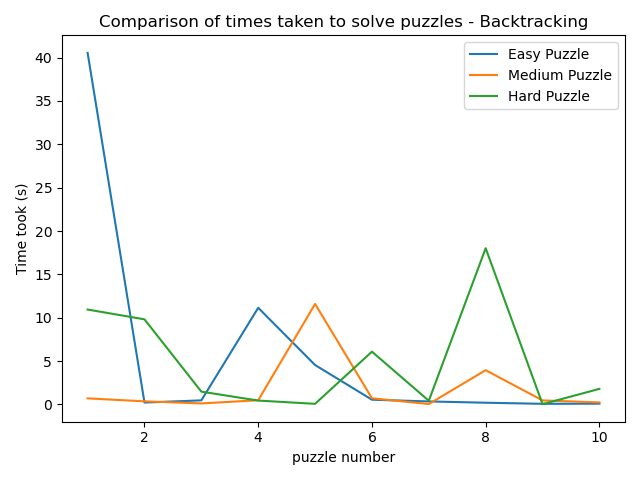
\includegraphics[width=75mm,scale=1]{figures/Backtracking.png}
\caption{Time Taken to Solve Each Difficulty-level of Sudoku Puzzles Using Backtracking}
\label{fig:backtrack_time}
\end{figure}

\subsubsection{Convolution Neural Network:}
An already available Sudoku dataset \cite{bib_cnndataset} of one million puzzles was used to train the CNN model. We split the dataset with a 95\%:5\% training data to test data ratio. Our CNN model records/saves the model after each epoch as a checkpoint and stops the epoch if the accuracy of the model appears to be decreasing compared to the previous epochs. We trained the model for 10 epochs and plotted the accuracy and loss for our trained model, shown in Fig. \ref{fig:accuracy_loss}. Most of the puzzles from the "Hard" category took the highest time to reach the solved state.

\begin{figure} [htbp]
\centering
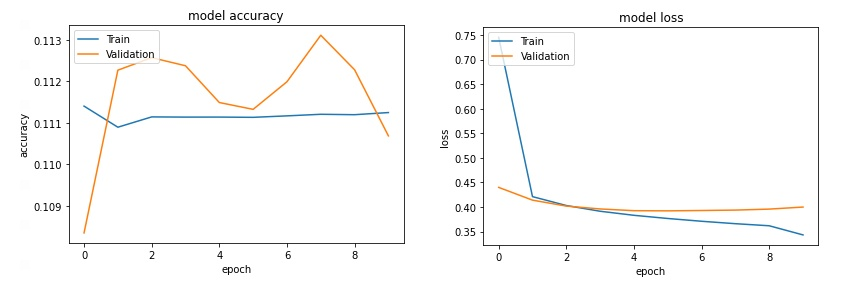
\includegraphics[width=90mm,scale=1.2]{figures/accuracy_loss.jpg}
\caption{Accuracy and Loss plot for the CNN trained model}
\label{fig:accuracy_loss}
\end{figure}
 

From Fig. \ref{fig:accuracy_loss}, we can deduce that the accuracy of the model is quite lower than expected, but that is most likely due to the reason that the Sudoku puzzles can be solved in multiple ways but we had only one answer per puzzle available in the dataset.

\begin{figure} [htbp]
\centering
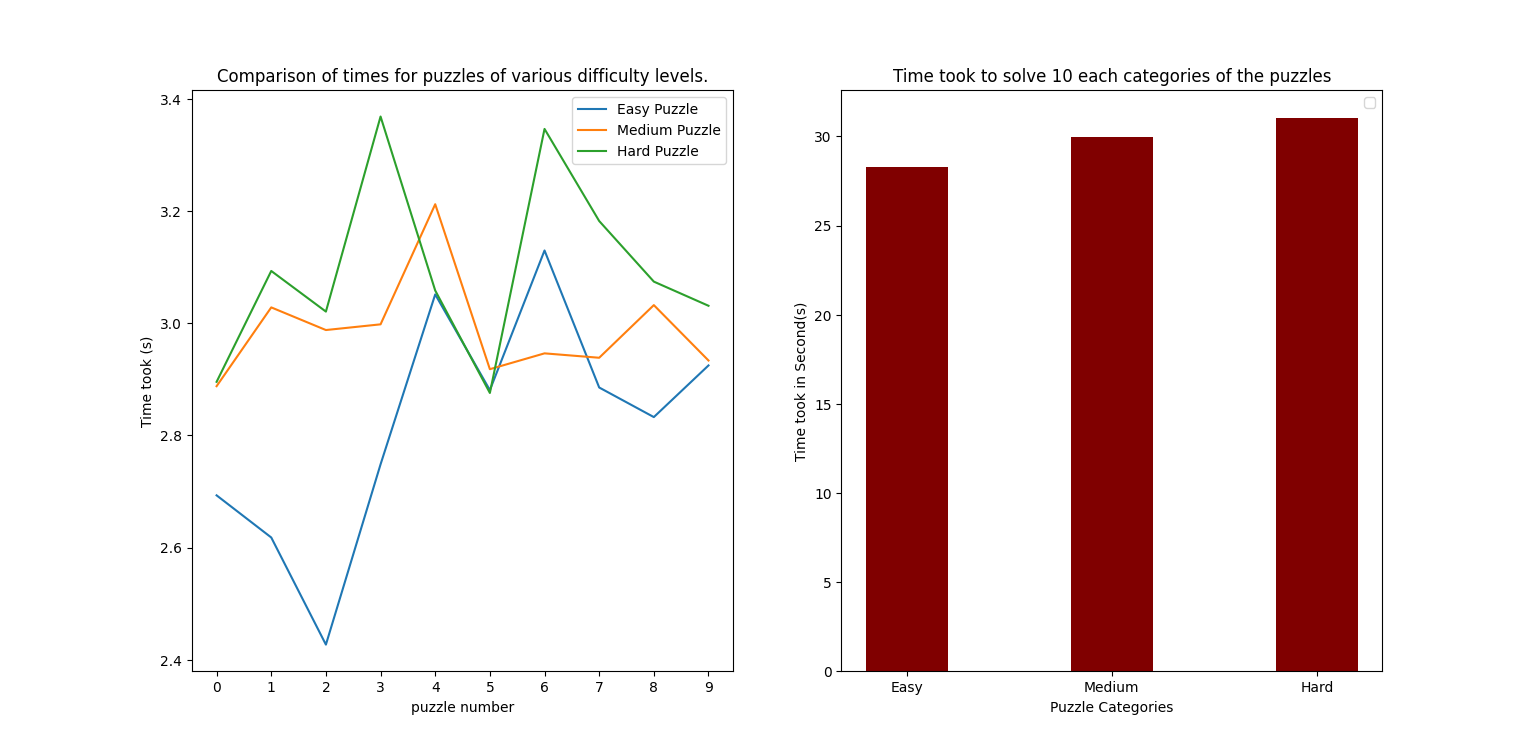
\includegraphics[width=120mm,scale=1.5]{figures/CNN_Analysis.png}
\caption{Time took for solving each categories of the puzzles}
\label{fig:cnn_difficulty_levels}
\end{figure}

From Fig. \ref{fig:cnn_difficulty_levels}. we can observe that the CNN model took least time in solving the “Easy” category of puzzles with lesser time gap when compared to “Medium” and “Hard” puzzles.

\subsubsection{Constraint Satisfaction:}
As mentioned earlier, Sudoku puzzle is fundamentally a constraint satisfaction problem. Using Pulp package, we defined the variables and the constraint of the given Sudoku puzzle. We then formulated the problem using linear programming. As it can be seen in Fig. \ref{fig:time_eval} and Fig. \ref{fig:memory_eval}, this method outperforms all the other algorithms insofar as the time taken to solve the puzzles is concerned. The Constraint Satisfaction agent has been able to solve any given Sudoku puzzle in the order of milliseconds. The memory usage is also relatively low compared to most of the other proposed agents. Given the fact that this agent does not require to be trained as opposed to CNN, this approach turned out to be the most efficient algorithm to be adopted to solve Sudoku puzzles.

\subsubsection{Genetic Algorithm:}

From the Fig. \ref{fig:ga_result}, we see that the time of searching for puzzle solutions on three different types of puzzles shows that the time of searching results on hard puzzles and simple puzzles are quite similar, but the time on the medium puzzle is higher than others. the reason for this may come from generated random collections of solutions with regard to mutation function. And the overall performance of the Genetic algorithm Genetic is time-consuming.

\begin{figure} [htbp]
\centering
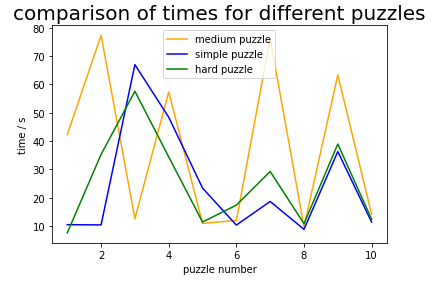
\includegraphics[width=90mm,scale=1]{figures/GA_result.png}
\caption{Comparison of times of three level puzzles using Genetic Algorithm}
\label{fig:ga_result}
\end{figure}

\subsubsection{Comparison with Baseline:}
As evident, all the algorithms performed exponentially better than the baseline algorithm of DFS. The Constraint Satisfaction algorithm did the best in terms of time taken. The Backtracking algorithm performed the best in terms of memory usage.